% Diese Zeile bitte -nicht- aendern.
\documentclass[course=erap]{aspdoc}

%%Packages
\usepackage{float}
\usepackage{tikz-qtree}
\usepackage{etoolbox}
\usetikzlibrary{trees}
\usepackage[edges]{forest}
\usepackage{colortbl}

\usepackage{pgfplots}
\pgfplotsset{width=7cm, compat=1.18}

\usepackage[symbol]{footmisc}
\renewcommand{\thefootnote}{\fnsymbol{footnote}}

\usepackage{tikz}
\tikzset{
  heap/.style={
    every node/.style={circle,draw},
    level 1/.style={sibling distance=30mm},
    level 2/.style={sibling distance=20mm}
  }
}
\usepackage{xcolor}
\usepackage[center]{caption}

\usepackage{pgfplots}
\pgfplotsset{width=7cm,compat=1.7}

\usepackage{caption}
\captionsetup[table]{name=Baum}
\captionsetup[table]{justification=raggedright,singlelinecheck=false}
%%%%%%%%%%%%%%%%%%%%%%%%%%%%%%%%%
%% TODO: Ersetzen Sie in den folgenden Zeilen die entsprechenden -Texte-
%% mit den richtigen Werten.
\newcommand{\theGroup}{294} % Beispiel: 42
\newcommand{\theNumber}{A404} % Beispiel: A123
\author{Wajih Tarkhani \and Michael Eichhorn \and Leonhard Obkirchner}
\date{Sommersemester 2023} % Beispiel: Wintersemester 2019/20
%%%%%%%%%%%%%%%%%%%%%%%%%%%%%%%%%



%%%%%%%%%%%%%%%%%%%%%%%%%%%%%%%%%

% Diese Zeile bitte -nicht- aendern.
\title{Gruppe \theGroup{} -- Abgabe zu Aufgabe \theNumber}

\begin
{document}
\maketitle

\section{Einleitung}
Die Datenkomprimierung spielt in verschiedenen Bereichen wie der Datenübertragung, Speicherung und Verarbeitung großer Datenmengen eine entscheidende Rolle. Angesichts steigender Datenmengen und begrenztem Speicherplatz ist es von großer Bedeutung, effiziente Methoden zur Reduzierung der Dateigröße zu entwickeln ohne dabei wesentliche Informationen zu verlieren. Durch die Anwendung von Kompressionsalgorithmen können große Datenmengen effizient codiert werden, um Platz zu sparen und die Übertragungsgeschwindigkeit zu verbessern. \\
Es gibt zwei grundlegende Arten von Datenkompression: verlustfreie und verlustbehaftete Kompression. Bei der verlustfreien Kompression werden die Daten so komprimiert, dass sie vollständig wiederhergestellt werden können, ohne dass Informationen verloren gehen. Dies ist besonders wichtig für Textdateien, Programmcode, Konfigurationsdateien etc...
Auf der anderen Seite ermöglicht die verlustbehaftete Kompression, indem irrelevante oder weniger wichtige Informationen entfernt werden.\\
\newline 
In diesem Projekt werden wir uns mit einem \emph{verlustfreien} Algorithmus beschäftigen: \emph{Huffman Algorithmus}.
Der Algorithmus basiert auf einem Huffman-Baum, der aus den Zeichen und ihren Häufigkeiten aufgebaut wird. Durch die Zuweisung von \emph{Binärcodes} zu den Zeichen wird die Effizienz der Kompression erreicht. Der Code enthält Funktionen zum \textbf{Codieren}
und \textbf{Dekodieren} von Daten mithilfe des Huffman-Baums. \\


\begin{lstlisting}[language=c, numbers=none, frame=none]
void huffman_encode(size_t len, const char[len] data)
\end{lstlisting}

\begin{lstlisting}[language=c, numbers=none, frame=none]
void huffman_decode(size_t len, const char[len] data)
\end{lstlisting}
Diese nehmen vom Benutzer spezifizierte Eingabestring bzw. das kodierte Datum \verb+data+ der Länge \verb+len+. Bei \verb+huffman_encode+ wird die Häufigkeitsanalyse durchgeführt, danach soll den Huffmanbaum konstruiert werden, um mit den einzelnen Bits an den Kanten die Eingabe binär zu kodieren. Bei \verb+huffman_decode+
wird der kodierte String mit dem kreierten Baum (oder mit dem erzeugten Dictionary) dekodiert.\\
\newline
Mit diesem Vorwissen mit dem Bezug zu der Aufgabenstellung kann sich nun in den folgenden Kapiteln mit Lösungsansätzen auseinandergesetzt, diese daraufhin auf ihre Korrektheit analysiert und anschließen auf ihre Performanz getestet werden. \\

\section{Lösungsansatz}
%%%%%%%%%%%%%%%%%%%%%%%%%%%%% ich habe nur das Beispiel geschrieben... in progress
Bevor wir uns mit der eigentlichen Implementierung auseinandersetzten können, müssen zunächst die
Rahmenbedingungen geklärt werden. Dafür ist es zwangsweise notwendig die Frage zu beantworten, welche Eingaben der Nutzer tätigen bzw. nicht tätigen darf. Laut Aufgabestellung ist es erwartet vom Nutzer eine Eingabedatei zur Verfügung zu stellen und mit \verb+-o+ eine Ausgabedatei zu wählen oder zu erstellen.
Und das gilt für die Kodierung und die Dekodierung, der einzige unterschied ist ,dass man bei der Dekodierung \verb+-d+ am Anfang hinzufügt. \\
Mit diesem definierten Rahmen haben wir die angegebenen Funktionssignaturen geändert, und zwar zwei neue Argumente hinzugefügt: \verb+outputFile+ und \verb+to_print+ \\ \\
\begin{lstlisting}[language=c, numbers=none, frame=none]
void huffman_encode(size_t len, const char data[len], FILE* outputFile, int to_print)
\end{lstlisting}
\begin{lstlisting}[language=c, numbers=none, frame=none]
void huffman_decode(size_t len, const char data[len], FILE* outputFile, int to_print)
\end{lstlisting}
 

\subsection{Lösungsansatz von Encode}\label{Encode}
Zunächst beschäftigen wir uns mit Encode. Wir betrachten dazu ein einfaches Beispiel mithilfe des Wortes \emph{ABRAKADABRAB}. \\
\newline
Ein gängigster Ansatz ist mit der Häufigkeitsanalyse anzufangen, indem wir die Häufigkeit der einzelnen Symbole in den Eingabedaten bestimmen indem wir ein \verb+int array+ dafür erstellen. \\
In diesem Frequenz-Array  wird für jeden Buchstaben im Buchstaben-Array seine Häufigkeit im Frequenz-Array erhöht. Dabei wird der \emph{ASCII-Wert} des Buchstabens als Index im Frequenz-Array verwendet. Das bedeutet, dass das Frequenz-Array so groß sein muss, wie die Anzahl der möglichen \emph{ASCII-Werte}. Die Häufigkeit der Buchstaben, die nicht im Buchstaben-Array vorkommen, bleibt bei \textbf{0}, da das Frequenz-Array zu Beginn mit Nullen gefüllt wurde.\\
\begin{figure}[H]
\centering
\captionsetup{justification=centering}
\begin{table}[H]
\centering

\begin{tabular}{|| c | c | c | c | c | c | c | c | c | c | c ||} 
 \hline
\rowcolor[gray]{0.9}   & ... & A & B & ... & D & ... & K & ... & R & ... \\ [0.5ex]
 \hline
Index (ASCII) & ... & 97 & 98 & ... & 100 & ... & 107 & ... & 114 & ...\\ [0.5ex]
\hline
Frequency & 0 & 5 & 3 & 0 & 1 & 0 & 1 & 0 & 2 & 0\\ [0.5ex]
\hline
\end{tabular}
\end{table}
\caption{Frequenz Array}
\end{figure}
Und jetzt von diesem langen array kreieren wir \emph{2 neue Arrays}: ein array für die \textbf{Buchstaben} ,die keine Nulle Frequenz haben, und ein array für  die \textbf{Frequenzen} ,die \textbf{größer} Null sind.
%\begin{figure}[H]
%\centering
%\captionsetup{justification=centering}
\begin{enumerate}
\begin{table}[H]
\centering
\item
\begin{tabular}{|| m{0.2\textwidth} | m{0.03\textwidth} | m{0.03\textwidth} | m{0.03\textwidth} | m{0.03\textwidth} | m{0.03\textwidth}||} 
 \hline
Characters & A & B & D & K & R \\ [0.5ex]
\hline
\end{tabular}
\item
\begin{tabular}{|| m{0.2\textwidth} | m{0.03\textwidth} | m{0.03\textwidth} | m{0.03\textwidth} | m{0.03\textwidth} | m{0.03\textwidth}||}  
\hline
Frequency & 5 & 3 & 1 & 1 & 2 \\ [0.5ex]
\hline
\end{tabular}
\end{table}
\end{enumerate}
%\caption{Buchstaben- und Frequenzen-Array}
%\end{figure}





%% array im Code als Tabelle zeichnen neben das menschen lesbarer Array 
Im nächsten Schritt bauen wir eine MinHeap-Datenstruktur als ein Array auf, wobei jeder Knoten bzw. jedes Element im Array ein \verb+MinHNode+ ist. Ein \verb+MinHNode+ enthält einen Buchstaben und seine Häufigkeit sowie zwei Zeiger auf das linke bzw. das rechte Kind.  \\
\begin{center}
\begin{tabular}{c}
\begin{lstlisting}[language=c, numbers=none, frame=none]
struct MinHNode{
  char character;
  unsigned freq;
  struct MinHNode* left;
  struct MinHNode* right;
};
\end{lstlisting}
\end{tabular}
\end{center}

\begin{enumerate}
\item Wir fügen alle Elemente in dem MinHeap array ohne die Reihenfolge zu beachten.
\begin{figure}[H]
\centering
\captionsetup{justification=centering}
\begin{table}[H]
\centering

\begin{tabular}{||c | c | c | c | c||} 
 \hline
A & B & D & K & R \\ [0.5ex]
 \hline
5 & 3 & 1 & 1 & 2 \\ [0.5ex]
\hline
\end{tabular}
\end{table}
\caption{Initialisierung von dem MinHeap-Array}
\end{figure}

%\vspace{\baselineskip}
\begin{figure}[H]
\centering
\captionsetup{justification=centering}
\begin{table}[H]
\item Wir führen jetzt \verb+set_up_MinHeap+ damit wir die MinHeap Invariante erstellen können.
\centering
%\vspace{\baselineskip} 
\begin{minipage}{0.4\textwidth} 
\begin{tabular}{||c | c | c | c | c||} 
 \hline
K & D & R & B & A \\ [0.5ex]
 \hline
1 & 1 & 2 & 3 & 5 \\ [0.5ex]
\hline
\end{tabular} 
\end{minipage} 
\quad
\vspace{\baselineskip} 
\begin{minipage}{0.4\textwidth} 
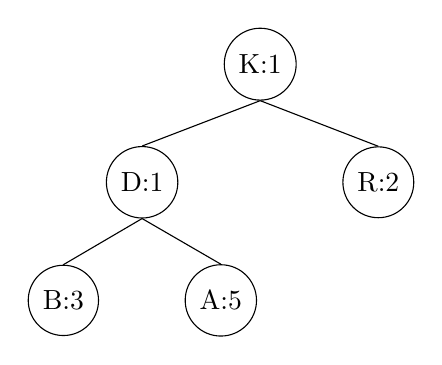
\begin{tikzpicture}[heap] 
\node {K:1}
  child{node{D:1}
    child{node{B:3}} child{node{A:5}}}
  child{node{R:2}}; 
\end{tikzpicture}
\end{minipage} 
\end{table}

\caption{MinHeap : Array und Baum Darstellung}
\end{figure}

\item Unser Ziel ist es einen \emph{präfix-freien}\footnote{Ein präfixfreier Baum wird verwendet, um eine Methode der sogenannten präfixfreien Codierung zu implementieren. Bei einer präfixfreien Codierung werden den einzelnen Symbolen eines Alphabets (zum Beispiel Zeichen oder Wörter) Bitmuster zugeordnet, so dass keine Bitfolge den Anfang einer anderen Bitfolge darstellt.} Baum (oder auch Huffman-Baum genannt) zu erstellen, mit dem wir ein sogenanntes \emph{Dictionary} erstellen werden.
%%%pop , insert und sift_down_up erklärt
Um den Huffman-Baum zu erstellen, können haben wir den fertigen MinHeap-Array als eine Prioritätswarteschlange betrachten, wo die Symbole nach ihrer Häufigkeit bereits sortiert sind. Dann können wir immer die zwei Symbole mit der niedrigsten Priorität aus der Warteschlange mit \verb+pop_Min()+ entfernen und einen neuen Knoten mit ihrer Summe als Priorität, das \verb+&+ als Character und die zwei Symbole als Kinder erstellen. Nach jedem \verb+pop_Min()+ rufen wir \verb+sift_down_up()+ auf, um die MinHeap Invariante wiederzustellen.
Jetzt fügen wir diesen Knoten wieder in die Warteschlange mit \verb+insert()+ ein. Wir wiederholen diese Schritte bis nur noch ein Knoten vorhanden ist. Dieser Knoten ist die Wurzel des Baumes.


\begin{table}[H]
        \centering
        \begin{tabular}{c}
            \toprule
            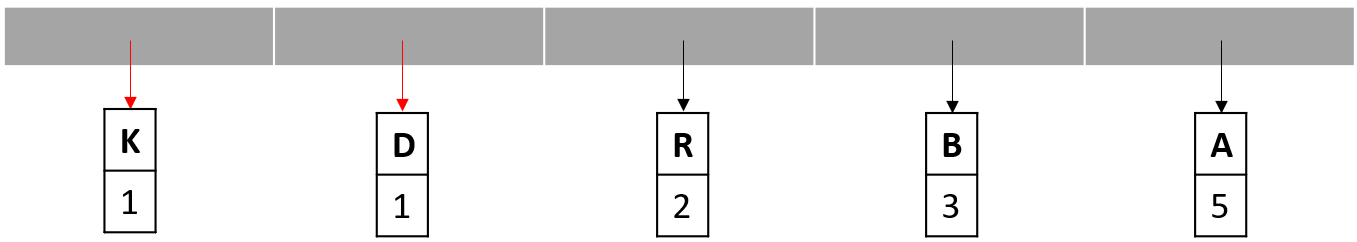
\includegraphics[width=12cm]{Abbildungen/Step0.png} \\
            \hline
            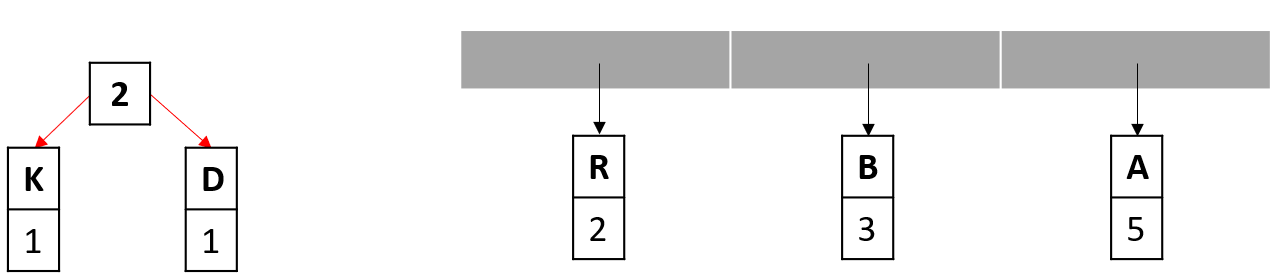
\includegraphics[width=10cm]{Abbildungen/Step1.png} \\
            \hline
            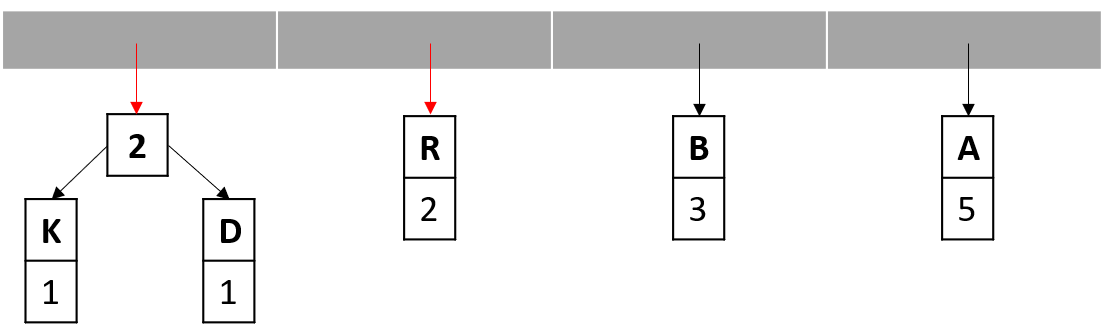
\includegraphics[width=10cm]{Abbildungen/Step2.png} \\
            \hline
            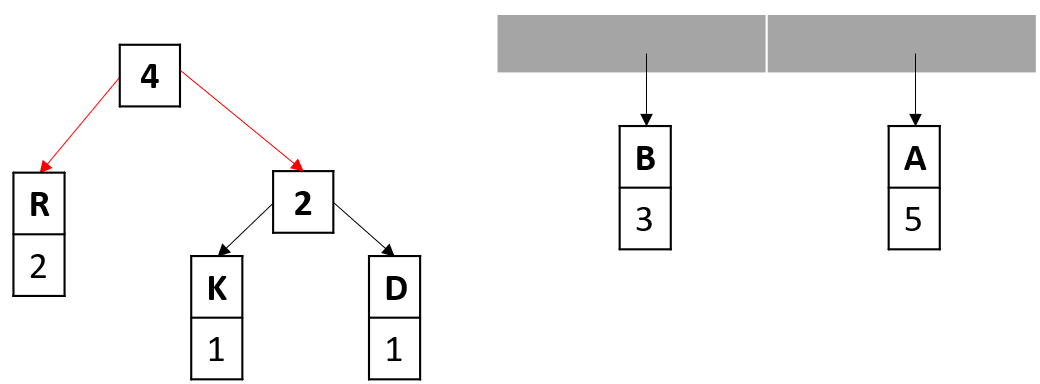
\includegraphics[width=10cm]{Abbildungen/Step3.png} \\
            %\bottomrule
        \end{tabular}
\end{table}
\begin{table}[H]
        \centering
        \begin{tabular}{c}
            %\toprule
            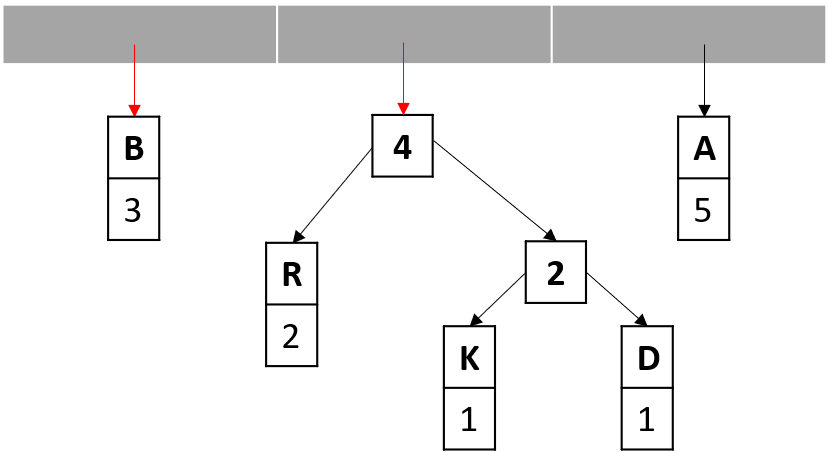
\includegraphics[width=10cm]{Abbildungen/Step4.png} \\
            \hline
            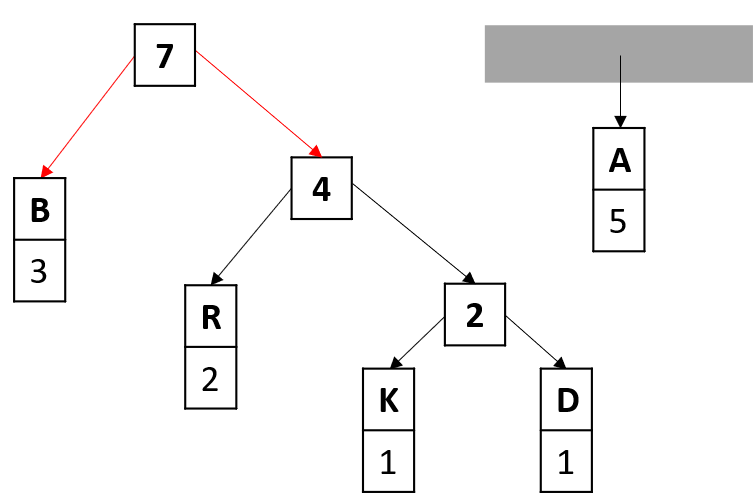
\includegraphics[width=8cm]{Abbildungen/Step5.png} \\
            \hline
            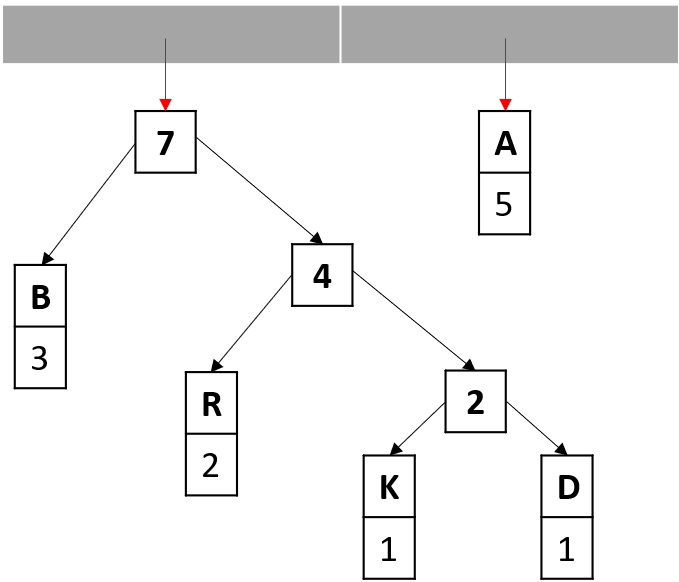
\includegraphics[width=8cm]{Abbildungen/Step6.png} \\
            \bottomrule
        \end{tabular}
\end{table}

\begin{center}
    Abbildung 4: Die Folge von \verb+pop_Min()+ und \verb+insert()+ Schritt für Schritt dargestellt
\end{center}

\vspace{5cm}
Und somit bekommen wir den \emph{präfix-freien} Baum, in welchem die häufigsten Symbole die kürzesten Codewörter zugewiesen bekommen.

%%note to self: das Begriff 'präfix-frei' erklären + die pop_min und sift_down_up erklären



\tikzset{iv/.style={draw,fill=white!50,circle,minimum size=20pt,inner
sep=0pt,text=black},ev/.style={draw,fill=yellow,rectangle,minimum
size=20pt,inner sep=0pt,text=black}}

\begin{forest}
for tree={where n children={0}{ev}{iv}, l+=3mm ,s sep=20mm, if n=1{edge label={node [midway, left] {0} } }{edge label={node [midway, right] {1} } },}
[12
 [A:5] 
 [7
  [B:3]
  [4
    [R:2]
    [2
        [K:1]
        [D:1]
    ]
  ]
 ] 
] 
\end{forest}


\item Der fertige Baum kann dann verwendet werden, um mit den einzelnen Bits an den Kanten die Eingabe binär zu kodieren. Dazu erstellt man das \emph{Dictionary}: \newline

\centering 
\begin{tabular}{||c | c||} 
 \hline
Symbol & Kodierung \\ [0.5ex]
 \hline
A & 0\\ [0.5ex]
\hline
B & 10\\ [0.5ex]
\hline
R & 110\\ [0.5ex]
\hline
K & 1110\\ [0.5ex]
\hline
D & 1111\\ [0.5ex]
\hline
\end{tabular}
\item Das gewählte Beispiel wird dann mithilfe der Tabelle buchstabenweise kodiert:\newline\newline
ABRAKADABRAB = 0 \space 10 \space 110 \space 0 \space 1110 \space 0 \space 1111 \space 0 \space 10 \space 110 \space 0 \space 10 \newline
\end{enumerate}
Anstatt 12 · 8 = 96 Bit zu benötigen, kann das Eingabewort mit 1 + 2 + 3 + 1 + 4 + 1 + 4 + 1 + 2 + 3 + 1 + 2 = 25 Bit kodiert werden. Zusätzlich zu diesen 25 Bit muss auch der Baum als Datenstruktur gespeichert werden, aber es ist klar, dass die Huffmankodierung bei längeren Texten eine hohe Kompressionsrate erzielen kann.

\subsection{Lösungansatz von Decode}\label{Decode}
Um die kodierten Daten zu dekodieren, gibt es zwei Ansätze: einen mit einem Dictionary und einen mit einem Baum.
Der Vorteil des Ansatzes mit einem Dictionary ist, dass er schneller sein kann, da er weniger Schritte benötigt, um ein Zeichen zu finden. Der Nachteil ist, dass er mehr Speicherplatz benötigt, um das Dictionary zu speichern oder zu übertragen, und dass er möglicherweise nicht funktioniert, wenn die Kodierung nicht \verb+präfix-frei+ ist. Der Vorteil des Ansatzes mit einem Baum ist, dass er weniger Speicherplatz benötigt, um den Baum zu speichern oder zu übertragen, und dass es immer funktioniert, egal ob die Kodierung \verb+präfixfrei+ ist oder nicht. Dazu ist er noch einfach zu implementieren, im Gegensatz zum ersten Ansatz. Der Nachteil ist, dass er langsamer sein kann, da er mehr Schritte benötigt, um ein Zeichen zu finden.
Wir haben uns entschieden, den zweiten Ansatz zu implementieren. Er funktioniert folgendermaßen:
\begin{enumerate}
    \item Man nimmt die kodierten Daten als eine Bitfolge und beginnt mit einem Zeiger auf die Wurzel des Baums.
    \item Man geht durch jedes Bit in der Bitfolge und bewegt den Zeiger entsprechend nach links oder rechts im Baum.
Wenn man auf einen Blattknoten stößt, hat man ein Zeichen gefunden, das man dekodieren will, und fügt es dem Ergebnis hinzu. Dann setzt man den Zeiger wieder auf die Wurzel.
    \item Man wiederholt den Prozess, bis man alle Bits in der Bitfolge verarbeitet hat.
\end{enumerate}

 




% TODO: Je nach Aufgabenstellung einen der Begriffe wählen
\section{Korrektheit}
Da es sich bei der Huffman-Codierung um eine verlustfreie Codierung handelt, wird im Weiteren nur die Korrektheit der Implementierung  betrachtet. Die Eingabe der Hauptfunktion \verb+huffman_encode+ wird nicht weiter beschränkt, solange diese ein String mit ASCII-Zeichen ist. Die Huffman-Codierung arbeitet zwar nicht auf den Werten der ASCII-Codierung, jedoch würde es den Rahmen des Projektes sprengen die Implementierung auf weitere Zeichen zu erweitern. Das Ergebnis der Hauptfunktion wird immer ein String sein, der sich aus dem Alphabet \{' ', '0', '1'\} zusammensetzt. Die zweite Hauptfunktion \verb+huffman_decode+ erwartet einen encodierten String aus Einsen und Nullen und wandelt diesen wieder in einen lesbaren String um. Ein zufälliger Binär-String kann nicht decodiert werden. Die korrekten Eingaben sind Vorraussetzung für eine erfolgreiche En- und Decodierung.

\subsection{Wichtigkeit des präfix-freien Baumes}
Die zentrale Eigenschaft des Huffman-Baumes ist, dass dieser immer \emph{präfix-frei} ist. Das bedeutet für die Implementierung, dass die verschiedenen ASCII-Zeichen immer in den Blättern gespeichert werden müssen. Ist dies nicht der Fall, ist die  Eindeutigkeit der Codierungen nicht mehr gegeben.

\begin{figure}[H]
\begin{table}[H]             
\centering 
\begin{minipage}{0.4\textwidth}
\tikzset{iv/.style={draw,fill=white!50,circle,minimum size=20pt,inner
sep=0pt,text=black},ev/.style={draw,fill=yellow,rectangle,minimum
size=20pt,inner sep=0pt,text=black}}
\begin{forest}
for tree={where n children={0}{ev}{iv}, l+=3mm ,s sep=5mm, if n=1{edge label={node [midway, left] {0} } }{edge label={node [midway, right] {1} } },}
[10
 [6
   [A:3]
   [E:3]
 ] 
 [4
   [B:2]
   [C:2]
 ] 
] 
\end{forest}
\caption{gültiger \\\hspace{0cm}Huffman-Baum}
\end{minipage}
\quad
\vspace{\baselineskip} 
\begin{minipage}{0.4\textwidth}
\tikzset{iv/.style={draw,fill=white!50,circle,minimum size=20pt,inner
sep=0pt,text=black},ev/.style={draw,fill=red,rectangle,minimum
size=20pt,inner sep=0pt,text=black}}
\begin{forest}
for tree={where n children={0}{ev}{iv}, l+=3mm ,s sep=5mm, if n=1{edge label={node [midway, left] {0} } }{edge label={node [midway, right] {1} } },}
[10
 [6
   [A:3]
   [E:3]
 ] 
 [B:4
   [C:2]
 ] 
] 
\end{forest}
\caption{ungültiger Huffman-Baum}
\end{minipage}
\end{table}
\end{figure}
Gegeben sind nun die Beispiele aus Baum 1 und 2, betrachtet wird der Teilstring 'ABC' zu den Huffman-Bäumen. Codiert man 'ABC' nach dem gültigen Baum ergibt sich das Dictionary \{A: 00, E: 01, B: 10, C: 11\} und folgender Code '001011'. Geht man nun zum ungültigen Baum über, fallen zwei Sachen auf. Einerseits steht ein ASCII-Zeichen in einer höheren Tree-Node und diese Tree-Node besitzt nur ein Kind. Es wird angenommen, dass die Node mit 'C' das linke Kind der Node mit 'B' ist. Daraus ergibt sich das Dictionary \{A: 00, E: 01, B: 1, C: 10\} und der Code '00110'. Würde der Code '00110' wieder decodiert werden, ergibt sich der String 'ABB' und je nach Implementierung kann ein Fehler geworfen werden. In diesem Beispiel erkennt man, dass die Codierung von 'B' ('1') ein Präfix der Codierung von 'C' ('10') ist. Daraus erschließt sich, dass jede Node mit einem gespeicherten ASCII-Zeichen ein Blatt sein muss, damit das Präfix-Problem nicht entsteht. Das impliziert, dass jeder Huffman-Baum ein voller Binär-Baum sein muss.
Beim Decodieren wird nur über den encodierten String iteriert und der aktuelle Code-String mit dem Dictionary verglichen.

\subsection{Analyse der Implementierung}
Hier wird überprüft, ob der generierte Huffman-Baum die Eigenschaften aus dem vorherigen Kapitel erfüllt. Für die Erstellung des Baumes ist die Funktion buildHuffmanTree mit folgender Signatur zuständig: \begin{lstlisting}[language=c, numbers=none, frame=none]
    struct MinHNode* buildHuffmanTree(char character[], int freq[], int size)
\end{lstlisting}
Der Funktion wird ein Array mit den unterschiedlichen ASCII-Zeichen und ein Array mit der jeweiligen Frequenz übergeben. Es wird jedes Zeichen mit zugehöriger Häufigkeit in einer Node gespeichert und einem MinHeap übergeben. Der Heap wird wie eine PriorityQueue benutzt. Über einen Pop-Befehl wird die Node mit der geringsten Frequenz entfernt und zurückgegeben. Entfernt man nun zwei Nodes mittels des Pop-Befehls und weist diese als Kinder einer neuen Node zu, kann man diese neue Eltern-Node wieder dem MinHeap hinzufügen. Hierbei ist es nicht möglich, dass eine schon vorhandene Node ein Parent einer anderen Node werden kann. Damit ist der Huffman-Baum automatisch ein voller Binärbaum und nur die Blätter enthalten die ASCII-Zeichen.
\newline
Um eine erfolgreiche Encodierung sicherzustellen, werden folgende Schritte überprüft. Nach der Erstellung des Huffman-Baumes wird mit einer simplen Rekursion über den Baum iteriert und falls die aktuelle Node ein Blatt ist, wird in einem Dictionary der zugehörige Pfad zum Blatt bzw. der Binär-Code gespeichert. Es wird danach nur noch über die Eingabe iteriert und die entsprechenden Codes der Zeichen in eine Ausgabedatei gespeichert.
\newline
Beim Decodieren wird wie beim Encodieren mithilfe der gespeicherten Daten wieder derselbe Huffman-Baum erstellt. Beim Durchlaufen des Codes wird je nach '0' oder '1' zum linken oder zum rechten Kind der aktuellen Node weitergegangen. Ist man bei einem Blatt angekommen, wird das gespeicherte ASCII-Zeichen ausgegeben und der Durchlauf beginnt wieder von vorne. Wenn der Huffman-Baum gültig ist, wird das Decodieren korrekt durchgeführt. Wird ein ungültiger Binär-String übergeben, gibt es dazu kein zugehöriges Dictionary und es wird bzw. kann nicht decodiert werden.




\section{Performanzanalyse}
Bevor wir mit der Performanzanalyse beginnen, sollte die Testumgebung spezifiziert werden. Alle Tests wurden auf einem \textbf{AMD Ryzen 7 5800H} Prozessor, 3.20 GHz, 16GB Arbeitsspeicher durchgeführt. Kompiliert wurde mit GCC 11.3.0 mit der Compiler-Stufe \textbf{O3}. Für jeden Messpunkt wurde die durchschnittliche Laufzeit aus 600 Funktionsaufrufen berechnet. Als Eingabewerte dafür dienten jeweils zwei zufällig generierte Strings aus allen druckbaren ASCII-Zeichen, woraus wiederum der Durchschnitt gebildet wurde. Da hier zwei voneinander getrennte Funktionen Encode und Decode vorliegen, untersuchen wir diese auch in Bezug auf Performanz unabhängig.

\subsection{Analyse von Encode}

\begin{center}
\begin{tikzpicture}
\pgfplotsset{every axis legend/.append style={at={(0,1)},anchor=north west}}
\begin{axis}[
    xlabel={$Anzahl\,Chars\,pro\,String\,$},
    ylabel={$Laufzeit\,in\,ms$},
    xmin=0, xmax=8000,
    ymin=0, ymax=5,
    xtick={0,2000,4000,6000,8000},
    ytick={0,1,2,3,4,5},
    grid=major,
    width=10cm,
    height=6cm
]

\addplot[color=red, mark=*] table {data/encode_V1Leo.txt};
\addplot[color=blue, mark=triangle] table {data/encode_V0Leo.txt};
\legend{$V0$, $V1$};

\end{axis}
\end{tikzpicture}
\end{center}Auf dem oberen Diagramm sind die Laufzeiten der Hauptimplementierung V0 und der Referenzimplementierung V1
bei variierender Länge der Eingabe-Strings verbildlicht. Die Referenzimplementierung verwendet die selbe Funktion zur Erstellung eines Huffmanbaums wie V0, sie unterscheidet sich jedoch im Bilden des Dictionaries grundlegend.\\
\,\,\,Wie man erkennen kann, nimmt die Ausführungsdauer bei V1 fast exponentiell zu, wohingegen sie bei V0 nur linear ansteigt. Wie weitere Tests ergaben, beruhen ca. 80\% der Laufzeit von V1 auf dem schlussendlichen Bilden des enkodierten Strings aus dem Dictionary, aus welchem Grund es Sinn macht diesen Teil zu optimieren, wie in V0 geschehen. Weil mit zufällig generierten Strings jeglicher Länge V0 schneller läuft, sollte diese Funktion bevorzugt werden.



\subsection{Analyse von Decode}

\begin{center}
\begin{tikzpicture}
\pgfplotsset{every axis legend/.append style={at={(0,1)},anchor=north west}}
\begin{axis}[
    xlabel={$Anzahl\,Chars\,pro\,String$},
    ylabel={$Laufzeit\,in\,\mu s$},
    xmin=0, xmax=8000,
    ymin=0, ymax=200,
    xtick={0,2000,4000,6000,8000},
    ytick={0,50, 100, 150, 200},
    grid=major,
    width=10cm,
    height=6cm
]
\addplot[color=blue, mark=triangle] table {data/decode.txt};

\end{axis}
\end{tikzpicture}
\end{center}Da beide Implementierungen die selbe Decode Methode verwenden, kann auch nur eine Funktion getestet werden. \\
Mit der Länge des Strings nimmt auch die Ausführungszeit von Decode linear zu.

\subsection{Interpertation der Performanzanalyse}
Da beide Funktion Encode\_V0 und Encode\_V1 die selbe Funktion beim bilden des Huffman-Baumes verwenden, widmen wir uns in diesem Teil den Unterschideden im Erstellen des Dictionaries.\\
Der Ansatz der V1 sieht folgendermaßen aus: Das Dictionary wird als Array der Länge 256 erstellt, wobei der Index als das als Zahl dargestellte ASCII-Zeichen zu interpretieren ist und der Wert die binär kodierte Version dieses Zeichens. Folglich bedeutet das, dass bei jedem Schreiben eines enkodierten Chars in den Ausgabe-String durch das Dictionary iteriert werden muss, um den passenden Index zu finden, im schlechtesten Fall sind das 256 Vergleiche.\\ 
Auf der unteren Abbildung ist ein Beispiel für ein solches Dictionary gegeben.\\
\begin{tabular}[h]{||l|c|c|c|c|c|c|c|c||}
\hline
\rowcolor[gray]{.9}Index & 0 & 1  & ...  & 113 & 114 & ...&254 & 255 \\
\hline
BinCode&\, & \,  & ... &  1111010 &  1110101 & ... & \, & \,   \\
\hline
\end{tabular}\\\\

Bei V0 hingegen ist das Dictionary-Array nur so lang, wie viele unterschiedliche Chars in dem Eingabe-String auch tatsächlich existieren. Es gibt also keinen Index, bei welchem das Char eine Häufigkeit von null aufweist, was bei V1 passieren kann. Die Einträge sind ein Struct, das einerseits das Char enthält und andererseits das enkodierte Ebenbild dessen.\\\\
\begin{tabular}[h]{||l|c|c|c|c|c|c|c|c||}
\hline
\rowcolor[gray]{.9}Index & 0 & 1  & ... & 47 & 48 & ...&88 & 89 \\
\hline
Char&   & A  & ...& k &  l  & ... & w & z   \\
\hline
BinCode& 1001010 &  1110111  & ... &   011110 &  111101 & ... &  1001000 & 100011   \\
\hline
\end{tabular}\\\\\\
Dadurch ist leicht ersichtlich, dass es effizienter sein muss, über ein in den allermeisten Fällen kleineres Array zu iterieren, als über eines, das konstant 256 groß ist.


 

\section{Zusammenfassung und Ausblick}
Die Ergebnisse des Projekts zeigen, dass Huffman-Codierung eine effektive Methode zur Datenkompression ist, die den Speicherplatz reduziert und die Übertragungszeit beschleunigt. Die Kompressionsrate hängt von der Häufigkeitsverteilung der Eingabezeichen ab. Je ungleichmäßiger die Verteilung ist, desto höher ist die Kompressionsrate. Rückblickend auf die Vorteile des Algorithmus, kann man sagen ,dass er eine optimale Methode zur Datenkompression ist. Außerdem ist er einfach zu implementieren und zu verstehen.
Und wie jeder Algorithmus hat die Huffmankodierung auch nachteile. Diese sind:
\begin{itemize}
\item Die Effizienz von Huffman-Codierung hängt von der Größe der Eingabedatei und der Anzahl der eindeutigen Zeichen ab. Je größer die Datei und je weniger Zeichen, desto effizienter ist die Kodierung.
\item Es erfordert einen zusätzlichen Speicherplatz für den Huffman-Baum oder die Tabelle, um die Kodierung zu speichern und wiederherzustellen.
\item Es ist nicht geeignet für Daten mit einer gleichmäßigen Häufigkeitsverteilung oder einer geringen Anzahl von Zeichen.
\end{itemize}

% TODO: Fuegen Sie Ihre Quellen der Datei Ausarbeitung.bib hinzu
% Referenzieren Sie diese dann mit \cite{}.
% Beispiel: CR2 ist ein Register der x86-Architektur~\cite{intel2017man}.
\bibliographystyle{plain}
\bibliography{Ausarbeitung}{}

\end{document}
